% LOCUS: supplementary material (IRO Journals template).
% Build: pdflatex locus_supplementary (named) or locus_supplementary_anonymous.
\documentclass[12pt,twoside]{article}
% Shared preamble of the LOCUS manuscript and its supplementary material (IRO Journals template).
\usepackage{geometry}
\usepackage[shortlabels]{enumitem}
\setlist{nosep}
\setlist[enumerate]{wide=0pt, widest=99,leftmargin=25pt, labelsep=*}
\usepackage[none]{hyphenat}
\usepackage{graphicx}
\graphicspath{ {./} }
\usepackage{titlesec}
\usepackage{booktabs}
\usepackage{mathptmx}
\usepackage{setspace}
\setlength{\parindent}{0pt}
\setlength{\parskip}{1em}
\sloppy
\usepackage{array}
\newcolumntype{P}[1]{>{\centering\arraybackslash}p{#1}}
\newcolumntype{M}[1]{>{\centering\arraybackslash}m{#1}}
\titleformat{\section}{\normalfont\fontsize{12}{12}\bfseries}{\thesection.}{12pt}{}
\titlespacing*{\section}{0pt}{12pt plus 2pt minus 2pt}{0pt}
\titleformat{\subsection}{\normalfont\fontsize{12}{12}\bfseries}{\thesubsection}{12pt}{}
\titlespacing*{\subsection}{0pt}{10pt plus 2pt minus 2pt}{0pt}
\geometry{a4paper, total={170mm,257mm}, left=2.54cm, top=2.65cm, right=2.54cm, bottom=2.65cm}
\rmfamily
\usepackage{fancyhdr}
\renewcommand{\footrulewidth}{0 pt}
\renewcommand{\headrulewidth}{0 pt}
% ---------------------------------------------------------------- additions needed by the content
\usepackage[T1]{fontenc}
\usepackage{amsmath,amssymb,multirow,xcolor,colortbl,tikz,microtype}
\usetikzlibrary{positioning,calc}
\usepackage[font=small,labelfont=bf,labelsep=period,skip=4pt]{caption}
\captionsetup[figure]{name=Figure}
\DeclareCaptionType[fileext=loa]{algo}[Algorithm][List of Algorithms]
\usepackage[numbers,square,sort&compress]{natbib}
\usepackage{placeins}
\usepackage[hidelinks]{hyperref}
\setlength{\textfloatsep}{8pt plus 2pt minus 2pt}
\setlength{\floatsep}{8pt plus 2pt minus 2pt}
\setlength{\intextsep}{8pt plus 2pt minus 2pt}
\renewcommand{\topfraction}{0.95}\renewcommand{\bottomfraction}{0.8}
\renewcommand{\textfraction}{0.05}\renewcommand{\floatpagefraction}{0.85}
\setcounter{topnumber}{4}\setcounter{bottomnumber}{3}\setcounter{totalnumber}{6}
\newcommand{\ours}{\textsc{LOCUS}}
\definecolor{bestc}{RGB}{200,235,200}\definecolor{secondc}{RGB}{210,225,248}
\newcommand{\best}[1]{\cellcolor{bestc}\textbf{#1}}
\newcommand{\second}[1]{\cellcolor{secondc}\underline{#1}}
\makeatletter\newcommand{\tabinput}[1]{\@@input #1 }\makeatother
\newcommand{\keywords}[1]{\par\textbf{\fontsize{12}{12}\selectfont Keywords:} #1}
\newcommand{\VLMFUNSD}{0.760}
\newcommand{\VLMIAM}{0.700}
\newcommand{\GAINIAMFone}{+0.027}
\newcommand{\GAINIAMauc}{+0.055}
\newcommand{\LOCUSCORDfone}{0.978}
\newcommand{\PQCORDfone}{0.973}
\newcommand{\PQIIITfone}{0.993}
\newcommand{\LOCUSIIITfone}{0.971}
\newcommand{\LOCUSSROIEfone}{0.973}
\newcommand{\PQSROIEfone}{0.742}
\newcommand{\LOCUSSROIEauc}{0.992}
\newcommand{\PQSROIEauc}{0.760}
\newcommand{\VLMSROIEfone}{0.866}

% Result-dependent sentences. Every number below is copied from the generated tables
% (tables/main_*_k25.tex, review_cost.tex, significance.tex, recog_*.tex, mp_analysis.tex,
% font_sensitivity.tex, char_error_subset.tex, audit.tex) after all runs finished.
\newcommand{\SROIESENTENCE}{On held-out SROIE the ranking of baselines flips: TrOCR's printed checkpoints were
fine-tuned on SROIE receipts, so TrOCR re-recognition is strong (.979 macro-F1) while PARSeq agreement fails on these
long receipt lines (.742); \ours{} is slightly below the former in macro-F1 (.973) and above it in AUROC (.992 vs.\ .978,
Table~\ref{tab:significance}). No single re-recognition baseline is the best choice on every dataset (PARSeq on forms
and scene text, TrOCR on SROIE, neither on handwriting), whereas \ours{} is within 0.006 macro-F1 of the best baseline
or better on four of the five datasets. Its average macro-F1 (.954) is the highest of all methods in
Table~\ref{tab:main}: well above the best single baseline (.907, PARSeq), equal to choosing the best baseline separately
for every dataset in hindsight (.954), and marginally above simple learners trained on our own counterfactual evidence
(.939--.952).}
\newcommand{\REVIEWSENTENCE}{At 95\% accepted precision, \ours{} requires reviewing 44.7\% of SROIE lines (TrOCR
re-recognition 45.0\%, PARSeq 69.5\%, the VLM judge 76.2\%, engine confidence 90.9\%) and 51.4\% of IAM words (PARSeq
54.6\%, the VLM judge 94.8\%). On FUNSD, CORD and IIIT5K, \ours{} and PARSeq are within two points of each other (FUNSD
37.2\% vs.\ 35.4\%, CORD 37.4\% vs.\ 38.6\%, IIIT5K 25.6\% vs.\ 25.3\%), while engine confidence and the VLM judge require
1.6--2.3$\times$ more review than \ours{} on the three receipt and form datasets. At the strictest target (98\%) PARSeq
is better on FUNSD and IAM.}
\newcommand{\XDSSENTENCE}{The ranking transfers well across all twenty dataset pairs (AUROC .892--.995;
e.g.\ FUNSD$\rightarrow$CORD .995 vs.\ .996 in-domain, CORD$\rightarrow$FUNSD .968 vs.\ .979). The weakest transfers are
those \emph{to} handwriting (SROIE$\rightarrow$IAM .892, CORD$\rightarrow$IAM .954) and from receipt lines to forms
(SROIE$\rightarrow$FUNSD .941). As for engines, macro-F1 at the fixed 0.5 threshold transfers much less well than the
ranking (e.g.\ SROIE$\rightarrow$FUNSD .620).}
\newcommand{\SIGSENTENCE}{Against the strongest baseline, \ours{} is significantly better on IAM in both metrics
($\Delta$AUROC $+0.055$, $\Delta$F1 $+0.026$, $p<0.001$), better in AUROC on CORD at the document level ($+0.007$,
$p=0.023$; macro-F1 $+0.005$, not significant) and on SROIE ($+0.014$, $p<0.001$, while TrOCR re-recognition is
slightly better in macro-F1, $-0.006$, $p=0.002$); it is statistically tied with PARSeq on FUNSD at the document level
($p=0.25$ and $p=0.12$) and significantly worse than PARSeq on IIIT5K ($-0.004$ AUROC, $-0.021$ macro-F1). It is
significantly better than the VLM judge and than TrOCR re-recognition on every dataset except SROIE, where the latter is
in-domain.}
\newcommand{\MPSENTENCE}{Three observations explain the null effect of message passing. First, removing message
passing changes neither metric by more than 0.009 on any dataset (A vs.\ B). Second, the \emph{explicit} comparison of each
rival with the claim does matter: removing the claim-relative features costs 0.010 to 0.023 macro-F1 on CORD, SROIE and
IIIT5K (A vs.\ C), and adding message passing back does not recover it (C vs.\ D). The network is not learning the
comparison from the graph; it uses the comparison when it is computed for it. Third, the graph is a depth-one star whose
readout already pools over every rival, so a message-passing layer can only re-express information the readout sees
anyway. Removing the rivals entirely (E) costs ranking quality on FUNSD (AUROC .974 to .961) but little elsewhere,
because the claim node keeps its own evidence and its agreement with both verifiers' readings, which summarise what the
strongest rivals would say. In short, what helps is counterfactual \emph{evidence}: scoring the claim against
alternatives under prior-cancelled likelihoods and making the comparison explicit; the graph is a convenient container
for it, not the source of the gain.}
\newcommand{\FONTSENTENCE}{The trained model is insensitive to the rendering: across seven
renderings its macro-F1 varies by at most 0.005 on every dataset (FUNSD .937--.939, CORD .972--.977, IAM .919--.923), and
the AUROC of the claim's ratio alone by at most 0.011. The training-free rule is more sensitive (AUROC .920--.940 on FUNSD,
.919--.944 on IAM); it is best with a serif or monospaced font rather than our default sans-serif, which we did not tune, and
a handwriting-like font does not help on handwriting. A mismatched rendering is thus absorbed by learning; only the
label-free rule would benefit from choosing the font.}
\newcommand{\CHARSENTENCE}{The removed share is large on FUNSD (51\% of errors) and moderate on CORD, SROIE and IAM
(18--23\%); IIIT5K's canonical protocol already excludes such differences. \ours{}' AUROC changes by at most 0.011
(it rises slightly or is unchanged), and its ordering relative to the baselines is unchanged except that the VLM judge,
whose AUROC rises most (FUNSD .846 to .928, SROIE .941 to .982), is visibly penalised by these artefacts. The conclusions of
Sec.~\ref{sec:main_results} therefore do not rest on annotation conventions.}
\newcommand{\AUDITSENTENCE}{Two conclusions follow. First, fewer than half of \ours{}' apparent
mistakes are genuine verification errors on a correct label (42 of 100 sampled): 25 are label noise, 9 crop problems and
8 ambiguous, and on IIIT5K 16 of 20 are claims that count as correct only after the case-insensitive, punctuation-free
normalisation of the protocol (\emph{e.g.}\ \texttt{HoLLywooD} for an upper-case sign), which \ours{}, judging the exact
appearance of the string, rejects; this protocol mismatch, rather than a visual error, explains most of \ours{}' gap to
PARSeq agreement (which compares normalised strings) on IIIT5K. Second, the stratum ``errors that PARSeq agrees with''
consists mostly of cases where the claim matches what is visible: only 10 of 92 sampled words are genuine errors, against
46 label-noise and 21 crop problems, so low rejection rates there are not a weakness of either verifier. The genuine
failures that remain fall into two identifiable modes: rejecting correct short or case-ambiguous claims when PARSeq reads
another case (CORD: \texttt{Rp}, \texttt{x}, \texttt{Pop}), and accepting capitalisation errors in handwriting (IAM:
\texttt{pinkie}, \texttt{market}, \texttt{church}).}

\expandafter\ifx\csname ifanon\endcsname\relax\expandafter\let\csname ifanon\expandafter\endcsname\csname iffalse\endcsname\fi % anonymous wrapper sets \ifanon=\iftrue

% cross-document references: \sref{label} = number of a label in the other document
\makeatletter\newcommand{\sref}[1]{\@ifundefined{xr@#1}{\textbf{??}}{\@nameuse{xr@#1}}}\makeatother

\InputIfFileExists{j_xref_main}{}{}% numbers of main-article labels (generated by make_xref.py)
\renewcommand{\thesection}{S\arabic{section}}
\renewcommand{\thetable}{S\arabic{table}}\renewcommand{\thefigure}{S\arabic{figure}}
\begin{document}
\begin{singlespace}
\begin{center}
\fontsize{20}{24}\selectfont\textbf{Supplementary Material}\\[6pt]
\fontsize{16}{20}\selectfont\textbf{LOCUS: Verifying OCR by Local Optimality over Counterfactual String Graphs}
\end{center}
\vspace{12pt}
\ifanon
\begin{center}\fontsize{12}{14}\selectfont Anonymous Author(s)\end{center}
\else
\begin{center}\fontsize{12}{14}\selectfont\textbf{Shikhar Dubey$^{1}$, Sanhita Saxena$^{2}$}\\[4pt]
\fontsize{10}{12}\selectfont $^1$Intelligent Systems, School of Computing and Electrical Engineering, and
$^2$School of Mathematical and Statistical Sciences, Indian Institute of Technology Mandi, Himachal Pradesh, India\\
s24130@students.iitmandi.ac.in, s25008@students.iitmandi.ac.in\end{center}
\fi
\end{singlespace}
\fontsize{12}{12}\selectfont
\begin{onehalfspace}
This document supplements the article \emph{LOCUS: Verifying OCR by Local Optimality over Counterfactual String
Graphs}. It gives the implementation details needed for reproduction and the complete experimental record behind the
summaries of the main article; references without the prefix S (e.g.\ ``Table~3'') point to the main article, and numbered citations such as [6]
refer to its reference list. All
tables and figures are generated by scripts from the raw result files; no number was entered by hand.

\section{Benchmark construction}
\label{app:data}
\textbf{Crops.} FUNSD words are cropped from the page with a 2-pixel margin after rescaling
the LayoutLM-normalised boxes ($[0,1000]^2$) of the public Hugging Face release to pixel coordinates;
cropping with the raw values yields misaligned crops for almost every word (the Tesseract word error
rate is 99.8\% without the rescaling and 36.9\% with it). CORD words are cropped from the axis-aligned
bounding box of each word quadrilateral; the official train and validation receipts form the training
pool. SROIE, IAM and IIIT5K are distributed as crops. Crops narrower than 6 or shorter than 8 pixels,
and empty transcriptions, are discarded.

\textbf{Engines.} Tesseract~5.2 (LSTM engine, \texttt{--psm 7}, crops shorter than 32 px are
bicubically upscaled to 32 px) outputs the space-joined words it detects and their mean confidence.
TrOCR-small (\texttt{microsoft/trocr-small-printed} or \texttt{-handwritten}) decodes greedily; its
confidence is the mean token probability.

\textbf{Labels.} A claim is \textsc{Correct} iff it equals the ground truth after whitespace
normalisation (case-insensitive for IIIT5K). No other normalisation is applied, so case and punctuation
errors count as errors, as they do for any downstream consumer that copies the field verbatim.

\textbf{Caveats.} TrOCR's printed checkpoints were fine-tuned on SROIE receipts; the verifier
$V_1$ is therefore in-domain on SROIE, and TrOCR-small makes only 3--6\% errors there, which is why
SROIE uses Tesseract claims. Tesseract is degenerate on handwriting (93.9\% word error on IAM), which is
why IAM uses TrOCR-small claims.


\section{Counterfactual neighbourhood generation}
\label{app:graph}
\textbf{Confusion groups.} Substitutions are drawn from the groups
\texttt{O0oQDCc}, \texttt{Il1|!ij}, \texttt{5Ss\$}, \texttt{8B\&3}, \texttt{2Zz}, \texttt{6Gb}, \texttt{9gq},
\texttt{7T/}, \texttt{uvnUV}, \texttt{wW}, \texttt{.,:;'`"}, \texttt{-\_\textasciitilde=}, \texttt{()\{\}[]},
\texttt{aeo}, \texttt{hbk}, \texttt{rnm}, \texttt{cC(e}, \texttt{xX\%}, \texttt{yY}, \texttt{pP}, \texttt{fft}; at most two
alternatives per character are used.

\textbf{Algorithm.} Given claim $h$ and verifier readings $g_1$ (TrOCR) and $g_2$ (PARSeq):
\begin{enumerate}
\item add $g_2$ and $g_1$ (if different from $h$);
\item for each reading, add every single edit of $h$ suggested by its Levenshtein alignment to the
reading: substitution of an aligned mismatching character, deletion of an unaligned character of $h$,
insertion of an unaligned character of the reading;
\item for each position of $h$ (up to 32): a case flip, up to two confusion substitutions, and a deletion;
\item deduplicate, keep insertion order, and stop at $M=28$ neighbours.
\end{enumerate}
No step uses the ground truth. The share of real errors whose truth is a node of the graph is reported
in Table~\sref{tab:truth_in_graph}.

\textbf{Rendering.} $R(v)$ draws $v$ in Liberation Sans (metrically equivalent to Arial) at
$0.75\times$ the crop height (clamped to $[32,96]$ px), black on white, with a quarter-height margin. The
same rendering is fed to both verifiers. PARSeq scores the string restricted to its 94-character
charset and truncated to its maximum label length of 25.


\section{Label-free pretraining data}
\label{app:pretrain}
From the unlabeled training pool we keep images on which two independent engines produce the
identical string (Tesseract and TrOCR-small; TrOCR-small and TrOCR-base on IAM), shuffle them with a
fixed seed and keep at most 3{,}000. Each yields a pseudo-correct graph (the agreed string) and, if the
corruption changes the string, a pseudo-incorrect graph built around one or two random OCR-style edits:
confusable substitution (45\%), case flip (15\%), deletion (20\%) or insertion of a confusable character
(20\%). The repair target of a corrupted graph is the node holding the agreed string (when present).
Agreement is a proxy, not ground truth; its precision on the training pool is reported in
Table~\ref{tab:pretrain_stats}.

\begin{table}[htbp]\centering
\caption{Label-free pretraining sets. Precision of engine agreement is measured post hoc against the
ground truth of the training pool (never used for training).}
\label{tab:pretrain_stats}
\scriptsize\begin{tabular}{lcccc}\toprule
Dataset & agreeing images & graphs & precision of agreement & truth in graph (corruptions) \\\midrule
\tabinput{tables/pretrain_stats.tex}
\bottomrule\end{tabular}\end{table}


\section{Hyperparameters and baseline protocols}
\label{app:hparams}
\begin{table}[htbp]\centering\caption{Hyperparameters (identical for all datasets and all $k$).}
\scriptsize\resizebox{\linewidth}{!}{\begin{tabular}{ll}\toprule
Node features & $2\times11$ evidence + 7 claim deltas ($\tanh$-squashed) + 8 edit-kind + 1 position + 6 agreement (claim node)\\
Edge features & 8 edit kinds + sibling + path + self (one-hot)\\
GNN & 3 GATv2 layers, hidden 64, 4 heads, residual + LayerNorm, dropout 0.2\\
Readout & claim state, attention pool, max pool over rivals, $\beta\log P_{\mathrm{opt}}$ ($\beta$ learned)\\
Pretraining & 15 epochs, AdamW lr $10^{-3}$, wd $10^{-4}$, batch 64, $\lambda=0.5$\\
Few-shot fine-tuning & 300 steps, AdamW lr $3\cdot10^{-4}$, batch $\min(64,k)$, class-balanced BCE\\
Head selection & repeated stratified CV (3 repeats, $\le$5 folds) on the support only; fusion if $\min$ class $<5$\\
Anchored head & priors scaled $\times10$; residual $\ell_2$ LR, $C\in\{.003,.01,.03,.1,.3\}$ by CV on the support\\
Full supervision & 60 epochs, early stopping (patience 8) on a 15\% split of the training pool\\
Seeds & 0--4 (support sampling, initialisation, pretraining)\\
\bottomrule\end{tabular}}\end{table}

\textbf{Thresholds.} Engine confidence and the $\rho$-margin rule are thresholded at the value
maximising macro-F1 on the $k$-shot support (seed-specific). Agreement baselines are binary
(accept iff equal). The graded PARSeq score is $+c$ if PARSeq's reading equals the claim and $-c$
otherwise, where $c$ is PARSeq's sequence confidence (product of character probabilities); it is
thresholded at 0, which coincides with the binary decision.

\textbf{VLM judge prompt.} \emph{Does the image show exactly the text "\{claim\}" (same characters,
case and punctuation)? Answer yes or no.} The image is passed at its native resolution (upscaled to a
height of 56 px if smaller; Qwen2.5-VL pixel budget 32--256 visual tokens). The score is the
renormalised probability of \texttt{yes}/\texttt{Yes} versus \texttt{no}/\texttt{No} as the first
generated token.

\textbf{ConfidNet-style learned confidence.} A one-hidden-layer MLP (32 units, $\ell_2$ $10^{-2}$)
on the engine confidence and five likelihood statistics of the claim under TrOCR-base, trained on the
support set.


\section{Additional analyses and qualitative examples}
\label{app:extra}
\subsection*{Error types}
Table~\ref{tab:error_types} breaks down the detection rate (recall of truly incorrect claims) by the edit that
separates the claim from the truth. Operating points: \ours{} at $P=0.5$, PARSeq-graded at its natural
threshold, the VLM at 0.5, and engine confidence at its \emph{test-optimal} threshold (favourable to the baseline).
\begin{table}[htbp]\centering
\caption{Detection rate (\%) by error type; number of errors of that type in parentheses ($k=25$).}
\label{tab:error_types}
\scriptsize\setlength{\tabcolsep}{3pt}\begin{tabular}{llccccc}\toprule
Dataset & Method & substitution & insertion & deletion & case only & multi-edit\\\midrule
\tabinput{tables/error_types.tex}
\bottomrule\end{tabular}\end{table}

\subsection*{Claim length}
\begin{figure}[htbp]\centering
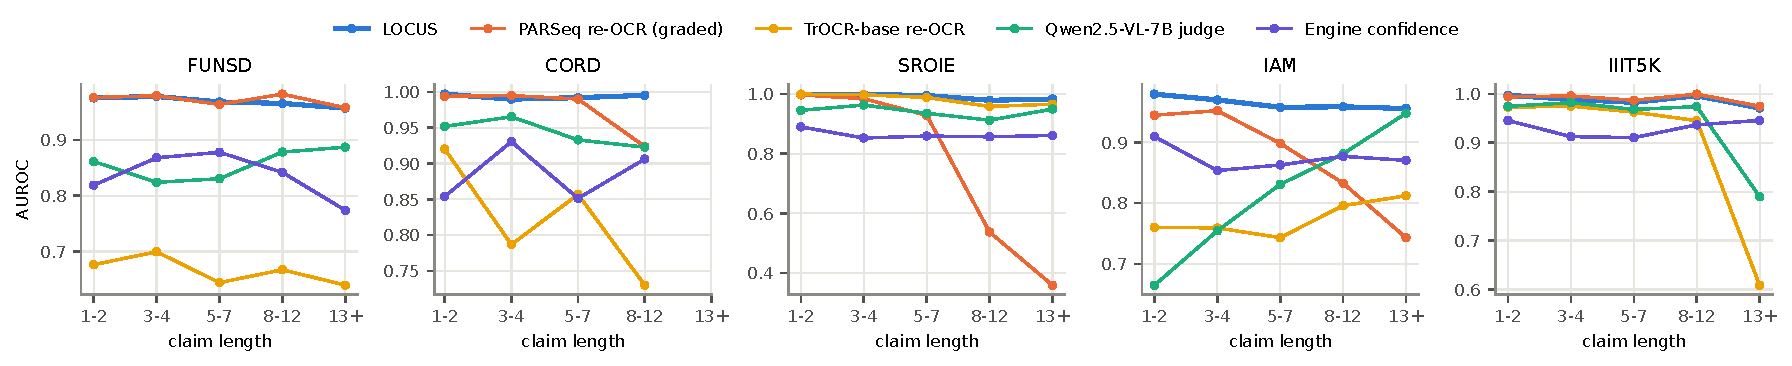
\includegraphics[width=\linewidth]{figs/by_length.pdf}
\caption{AUROC by claim length ($k=25$). Bins with fewer than 30 words or a single class are omitted.}
\label{fig:by_length}
\end{figure}

\subsection*{Calibration}
\begin{table}[htbp]\centering
\caption{Expected calibration error (15 bins) of the correctness probability ($k=25$; PARSeq-graded mapped
to $[0,1]$ as $(s+1)/2$). Lower is better.}
\label{tab:calibration}
\scriptsize\begin{tabular}{lcccc}\toprule
Dataset & \ours{} & PARSeq graded & Qwen2.5-VL-7B & Engine conf.\\\midrule
\tabinput{tables/calibration.tex}
\bottomrule\end{tabular}\end{table}

\subsection*{AUROC and AURC learning curves}
\begin{figure}[htbp]\centering
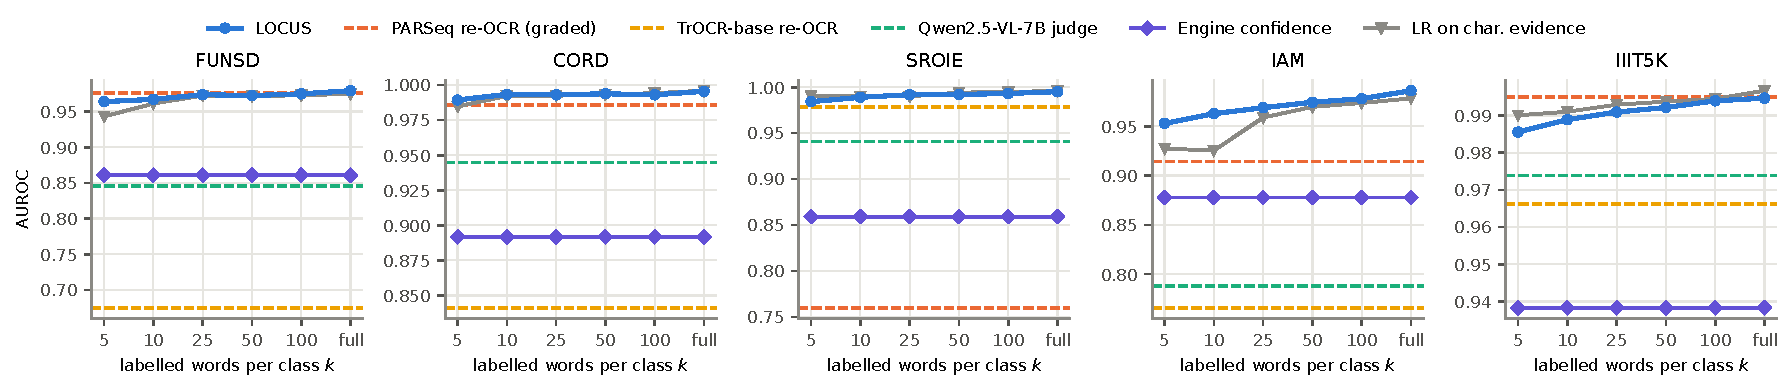
\includegraphics[width=\linewidth]{figs/learning_curves_auroc.pdf}
\caption{AUROC as a function of the number of labelled words per class (ensembles of five seeds;
dashed: label-free baselines).}
\label{fig:lc_auroc}
\end{figure}

\subsection*{Cross-dataset transfer (AUROC)}
\begin{table}[htbp]\centering
\caption{Cross-dataset transfer, AUROC (rows: training dataset, fully supervised; columns: test dataset;
diagonal: in-domain).}
\label{tab:xds_auroc}
\scriptsize\begin{tabular}{lccccc}\toprule
Train $\backslash$ Test & FUNSD & CORD & SROIE & IAM & IIIT5K\\\midrule
\tabinput{tables/xdataset_auroc.tex}
\bottomrule\end{tabular}\end{table}

\subsection*{Ablations: AUROC and repair}
\begin{table}[htbp]\centering
\caption{Ablations at $k=25$, AUROC (ensemble of five seeds). Last column: mean change w.r.t.\ the full model.}
\label{tab:ablation_auroc}
\scriptsize\begin{tabular}{lcccccc}\toprule
Variant & FUNSD & CORD & SROIE & IAM & IIIT5K & $\Delta$\\\midrule
\tabinput{tables/ablation_auroc.tex}
\bottomrule\end{tabular}\end{table}

\subsection*{Sensitivity}
\begin{table}[htbp]\centering
\caption{Sensitivity of \ours{} ($k=25$, ensemble of five seeds) to the size of the label-free pretraining
set, the number of fine-tuning steps, and the support-selection strategy (label-free $k$-means clusters the
unlabeled pool in the pretrained embedding space and labels the $2k$ medoids).}
\label{tab:sensitivity}
\scriptsize\begin{tabular}{llcccccc}\toprule
& & \multicolumn{2}{c}{FUNSD} & \multicolumn{2}{c}{CORD} & \multicolumn{2}{c}{IAM}\\
Factor & Value & F1 & AUROC & F1 & AUROC & F1 & AUROC\\\midrule
\tabinput{tables/sensitivity.tex}
\bottomrule\end{tabular}\end{table}

\subsection*{Main comparison at other label budgets and metrics}
\newcommand{\maintab}[3]{\begin{table}[p]\centering\caption{#2}\label{#3}
\scriptsize\setlength{\tabcolsep}{4pt}\resizebox{\linewidth}{!}{\begin{tabular}{lcccccc}\toprule
Method & FUNSD & CORD & SROIE & IAM & IIIT5K & Avg.\\\midrule
\tabinput{tables/#1.tex}
\bottomrule\end{tabular}}\end{table}}
\maintab{main_macro_f1_k10}{Macro-F1 at $k=10$ (protocol of Table~\sref{tab:main}).}{tab:main_f1_k10}
\maintab{main_macro_f1_k100}{Macro-F1 at $k=100$.}{tab:main_f1_k100}
\maintab{main_macro_f1_kfull}{Macro-F1 with full supervision (85\% of the training pool; 15\% for early stopping).}{tab:main_f1_full}
\maintab{main_auroc_k10}{AUROC at $k=10$.}{tab:main_auc_k10}
\maintab{main_auroc_k100}{AUROC at $k=100$.}{tab:main_auc_k100}
\maintab{main_aurc_k25}{AURC at $k=25$ (lower is better; best = lowest).}{tab:main_aurc_k25}
\maintab{main_cov@95_k25}{Coverage at 95\% accepted precision at $k=25$ (higher is better).}{tab:main_cov_k25}

\subsection*{Composition of real OCR errors}
\begin{figure}[htbp]\centering
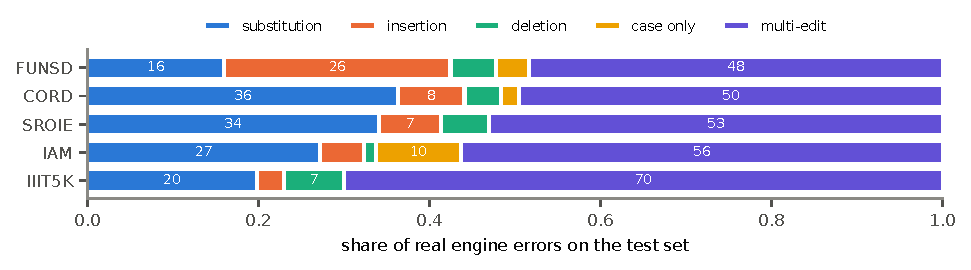
\includegraphics[width=0.85\linewidth]{figs/error_type_dist.pdf}
\caption{Types of real engine errors on each test set (share of errors; labels for shares above 7\%).
Handwriting and receipt lines are dominated by multi-edit errors, which bounds what a single-edit
neighbourhood can repair (Table~\sref{tab:truth_in_graph}).}
\label{fig:error_type_dist}
\end{figure}

\begin{figure}[htbp]\centering
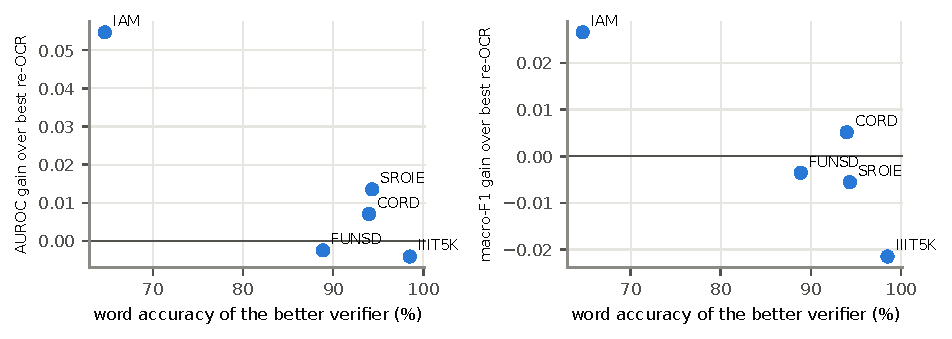
\includegraphics[width=0.75\linewidth]{figs/recog_dependence.pdf}
\caption{Gain of \ours{} over the best re-recognition baseline against the word accuracy of the better verifier (one
point per dataset).}
\label{fig:recog}
\end{figure}
\begin{figure}[htbp]\centering
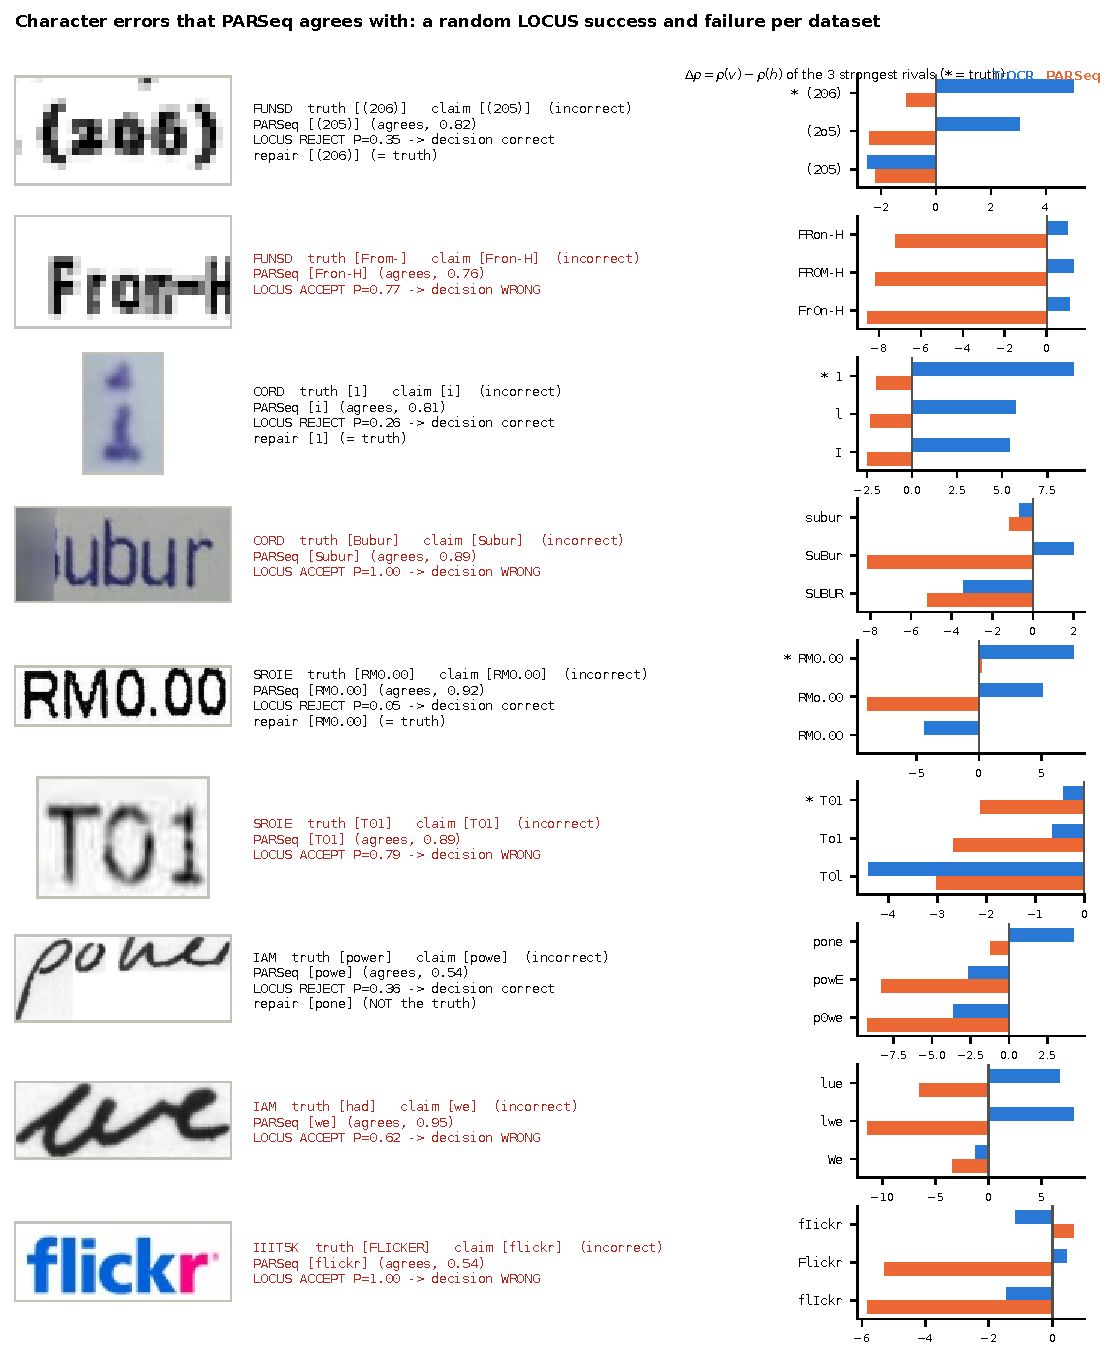
\includegraphics[width=0.8\linewidth]{figs/qual_regime_fooled.pdf}
\caption{\textbf{Errors that PARSeq re-recognition accepts} (it reads the same string as the engine), restricted to
genuine character errors (case-only and punctuation-only differences excluded): for each dataset one random
\ours{} success and one random failure. \ours{} rejects only a small fraction of this stratum
(Table~\sref{tab:qual_counts}); the manual audit (Table~\sref{tab:audit}) shows why: most of these ``errors'' are
annotation or cropping problems, i.e.\ the claim matches what is visible.}
\label{fig:qual_fooled}
\end{figure}

\begin{figure}[htbp]\centering
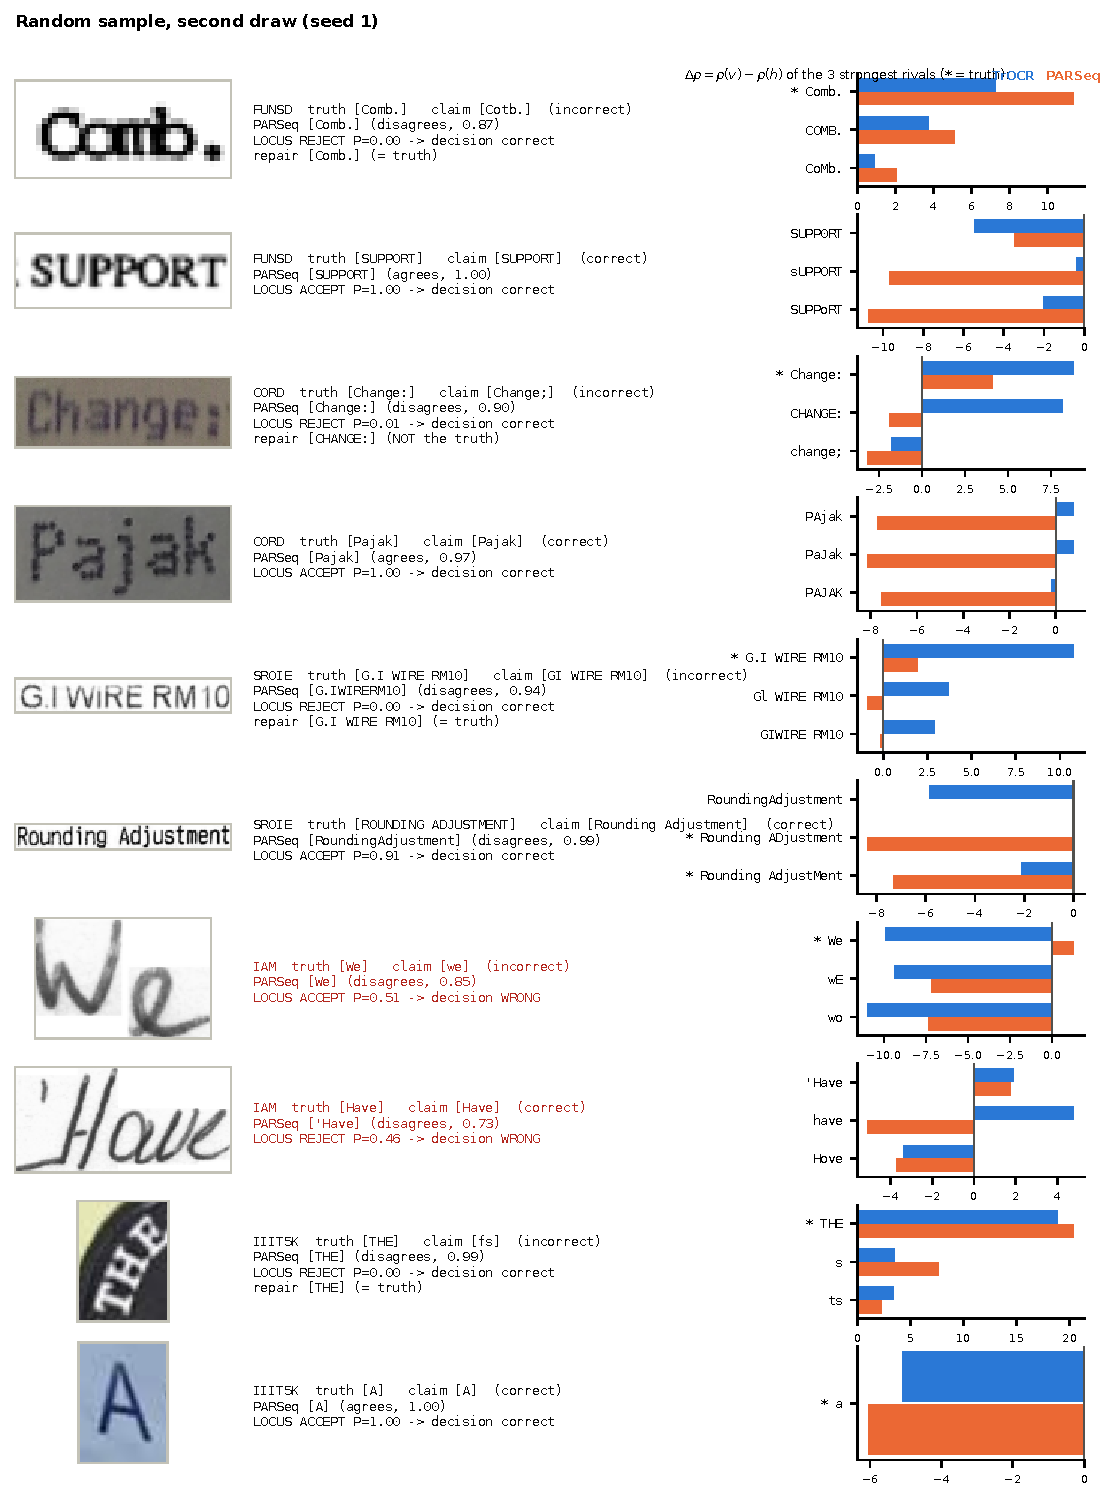
\includegraphics[width=0.8\linewidth]{figs/qual_random2.pdf}
\caption{\textbf{Second random sample} (seed 1), same protocol as Fig.~\sref{fig:qual_random}.}
\label{fig:qual_random2}
\end{figure}

\begin{figure}[htbp]\centering
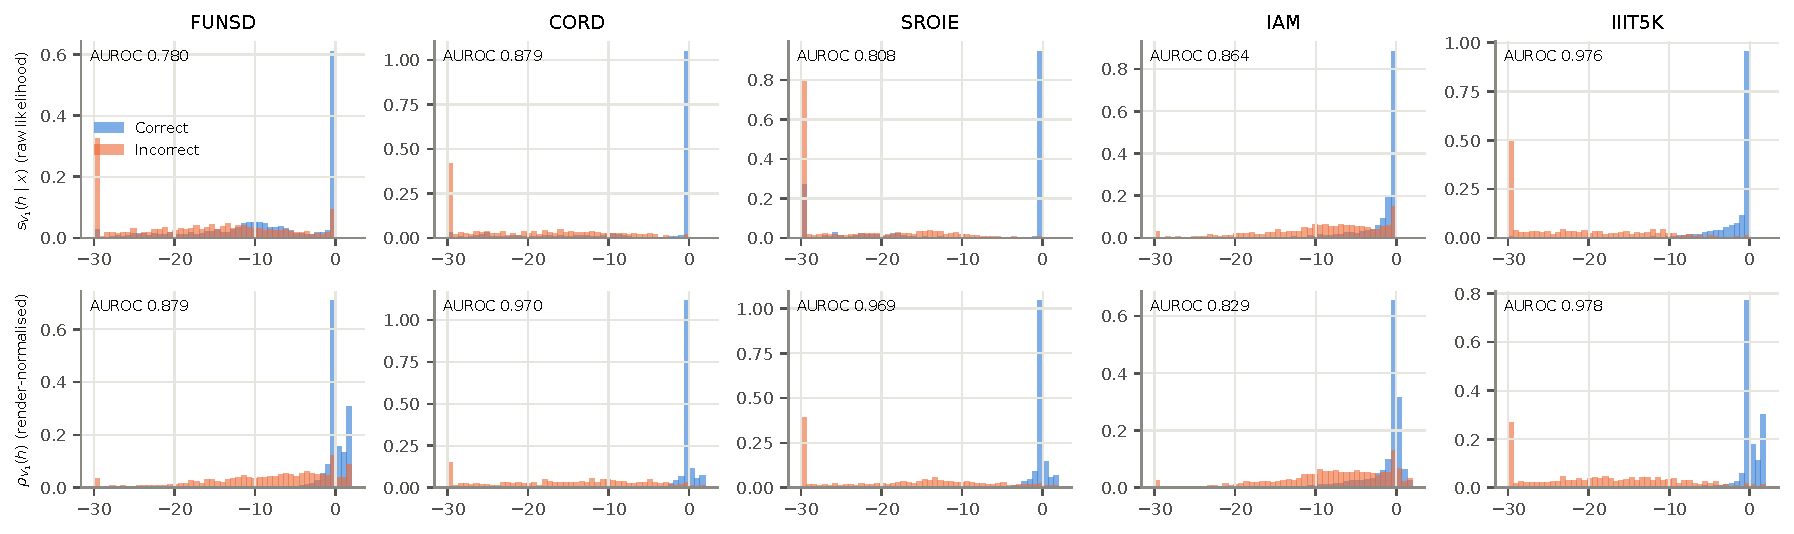
\includegraphics[width=0.92\linewidth]{figs/rho_separation.pdf}
\caption{\textbf{Render normalisation on real data.} Distribution of the claim's raw TrOCR likelihood (top) and of its
render-normalised ratio $\rho$ (bottom) for correct and incorrect claims, with the AUROC of each single score.}
\label{fig:rho}
\end{figure}

\begin{table}[htbp]\centering
\caption{\textbf{Single-verifier setting} (no agreement features), $k=25$, macro-F1: effect of render normalisation
when only one recogniser is available.}
\label{tab:single}
\footnotesize\begin{tabular}{lccccc}\toprule
Variant & FUNSD & CORD & SROIE & IAM & IIIT5K\\\midrule
\tabinput{tables/ablation_single.tex}
\bottomrule\end{tabular}\end{table}

\section{Full results}
\label{app:full}
Tables~\ref{tab:k_macro_f1_FUNSD}--\ref{tab:all_IIIT5K_k25} report every method at every $k$ with seed standard
deviations, and every metric at $k=25$.

\tabinput{tables/kgrid_macro_f1.tex}
\tabinput{tables/kgrid_auroc.tex}
\tabinput{tables/all_metrics_k25.tex}

\end{onehalfspace}
\end{document}
